\section{Evaluation}

\subsection{Evaluating Results}
\label{subsec:Evaluating Results}

\noindent
Model performance was assessed using the metrics defined in the Phase 4 test design. The table below presents the evaluation results for all three models on the held-out test set.

\begin{table}[ht]
\centering
\small
\begin{adjustbox}{max width=\textwidth}
\begin{tabular}{|l|r|r|r|r|r|r|r|}
\hline
\hline
Model & MAE & MSE & RMSE & R\textsuperscript{2} & ASE & SSE & ObservedAvg\\
\hline
Random Forest & 35.58 & 5978.4 & 77.32 & 0.946 & 5978.4 & 169913246.5 & 1016.17\\
HistGradientBoosting & 47.07 & 7344.9 & 85.70 & 0.934 & 7344.9 & 208749725.6 & 1016.17\\
XGBoost & 46.47 & 6820.1 & 82.58 & 0.939 & 6820.1 & 193833558.3 & 1016.17\\
\hline
\hline
\end{tabular}
\end{adjustbox}
\caption{Model Performance Metrics Comparison}
\label{tab:model_performance}
\end{table}

\noindent
Random Forest achieved the highest R\textsuperscript{2} of 0.946 and the lowest error metrics across all categories, indicating the strongest predictive performance among the three models. XGBoost ranked second with an R\textsuperscript{2} of 0.939, while HistGradientBoostingRegressor achieved an R\textsuperscript{2} of 0.934. All three models performed well, with the gap between the best and worst model being only 0.012 in R\textsuperscript{2}.

\noindent
For this project, these results mean that Random Forest is the strongest candidate for estimating rental prices from listing data. Its performance suggests that the model can produce predictions reasonably close to actual prices for many properties in the dataset, making it the most reliable of the three tested approaches. The Observed Average price of \$1,016.17 provides a meaningful baseline: Random Forest's MAE of \$35.58 represents an average prediction error of approximately 3.5\% relative to the mean listing price, which is a strong result for this domain. This is important because the main goal of the project is to produce a predictive understanding of what drives apartment listing prices in the Southern United States.

\noindent
The feature importance results confirm that location-based features are the dominant drivers of rental price. The location\_cluster feature created by K-Means clustering on latitude and longitude coordinates ranked as the most important predictor across all three models. Region and square footage (sqfeet) consistently appeared in the top three. Table \ref{tab:fi_ranking} summarises the top features and their rankings across all three models.

\begin{table}[ht]
\centering
\small
\begin{tabular}{|l|c|c|c|}
\hline
\hline
Feature & RF & HistGB & XGB \\
\hline
location\_cluster & 1 & 1 & 1 \\
region & 2 & 3 & 2 \\
sqfeet & 3 & 2 & --- \\
lat & 4 & --- & --- \\
long & --- & 4 & --- \\
baths & --- & --- & 3 \\
laundry\_options & --- & --- & 4 \\
\hline
\hline
\end{tabular}
\caption{Feature importance rankings across models (blank = outside top 4)}
\label{tab:fi_ranking}
\end{table}

\noindent
The cross-model agreement is notable: location\_cluster is the most important predictor in every model, confirming that geographic clustering captured meaningful price variation that individual region labels alone could not. For renters, this means the model can help assess whether a property is reasonably priced relative to its area and size. For landlords and property managers, it shows which factors have the greatest influence on expected rental value, and that individual amenities such as laundry options or pet policies matter far less than location and size.

\begin{figure}[h!]
    \centering
    \caption{Observed vs Predicted Values}
    \label{fig:OvP}

    \begin{subfigure}[b]{0.329\textwidth}
        \centering
        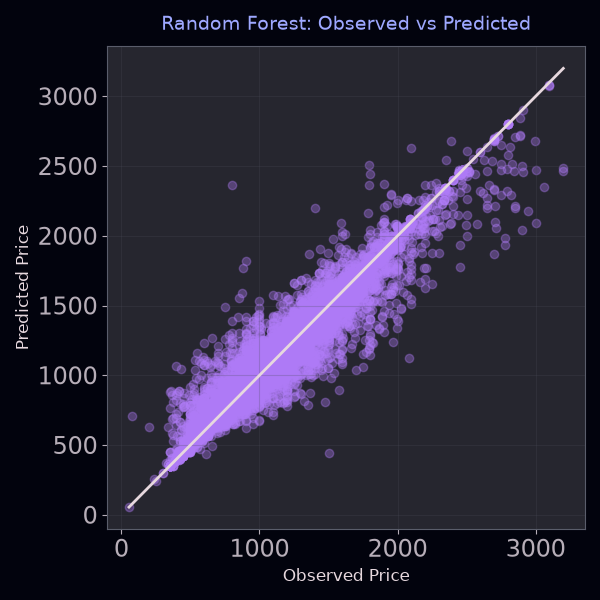
\includegraphics[width=\textwidth]{Assignment/Phase5/charts/Random Forest: Observed vs Predicted.png}
        \caption{Random Forest}
        \label{fig:OvP_RF}
    \end{subfigure}
    \hfill
    \begin{subfigure}[b]{0.329\textwidth}
        \centering
        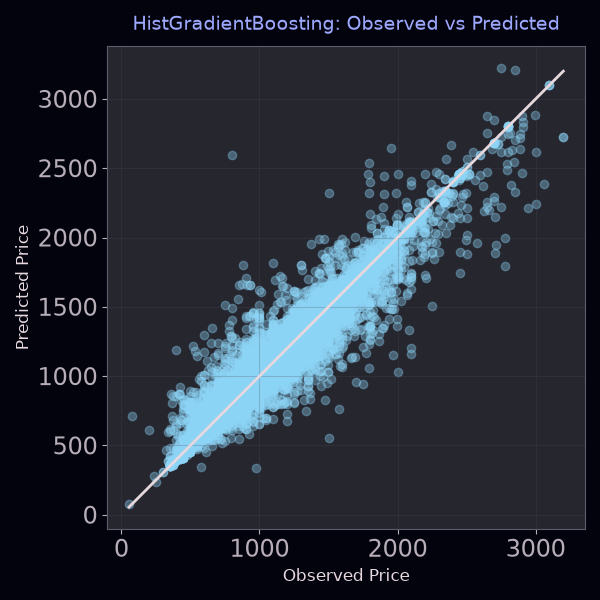
\includegraphics[width=\textwidth]{Assignment/Phase5/charts/HistGradientBoosting: Observed vs Predicted.png}
        \caption{HistGradientBoosting}
        \label{fig:OvP_GB}
    \end{subfigure}
    \hfill
    \begin{subfigure}[b]{0.329\textwidth}
        \centering
        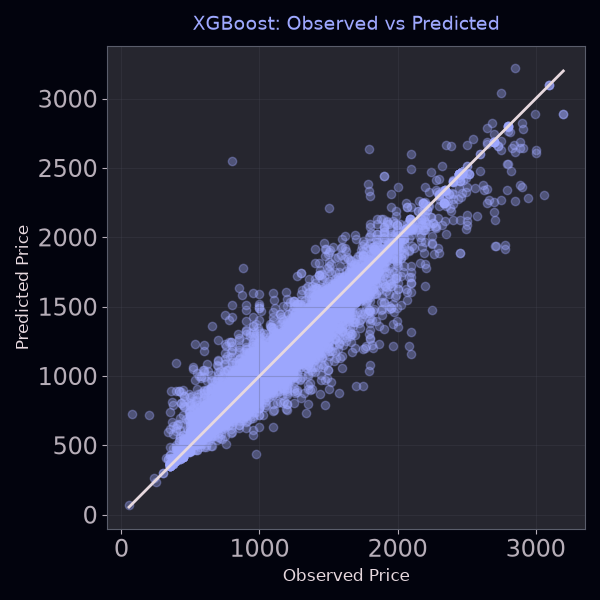
\includegraphics[width=\textwidth]{Assignment/Phase5/charts/XGBoost: Observed vs Predicted.png}
        \caption{XGBoost}
        \label{fig:OvP_XGB}
    \end{subfigure}
\end{figure}

\noindent
The observed-versus-predicted plots (Figure \ref{fig:OvP}) further support the usefulness of the modeling approach, since most predictions follow the general trend of the actual values. However, a slight broadening of the spread at higher price levels suggests that the models are less precise for the most expensive listings. This indicates the project shows strong promise, but is not yet ready for deployment without further tuning and validation.

\subsection{Reviewing the Process}

\noindent
The process review captures several important lessons from the project.

\noindent
First, the initial modeling iterations did not use K-Means for location clustering, and the results were noticeably weaker. Adding location clustering around Craigslist-defined regions (n\_clusters=148) substantially improved model performance. The location\_cluster feature emerged as the number-one predictor across all three models, confirming that this engineering decision was one of the most impactful of the project.

\noindent
Second, the project initially applied IQR-based outlier handling at the national level. After changing the procedure to apply IQR filtering by individual region, the models improved notably. This indicates that region-sensitive cleaning better reflected the structure of the housing market data, where price distributions vary meaningfully between different metropolitan areas.

\subsection{Determining the Next Steps}

\noindent
The following potential improvements were identified for future iterations of this project:

\vspace{-12pt}
\begin{itemize}[itemsep=-9pt]
    \item Optimize K-Means clustering by systematically finding the optimal number of clusters (e.g., elbow method or silhouette scores) rather than matching the number of Craigslist regions.
    \item Using newer and larger datasets would improve model relevancy to current market forces and expand geographic coverage beyond the Southern USA.
    \item Applying NLP to the description field could reveal insights missed by structured features, such as renovation quality or neighborhood character.
    \item Use GPU/CUDA to speed up training, tuning, and hyperparameter search for more extensive experimentation.
    \item Combining all three models in a weighted ensemble could improve prediction reliability by leveraging the strengths of each approach.
    \item Additional feature engineering (such as price-per-square-foot ratios, proximity to urban centers, or property age estimation) could capture further explanatory power.
\end{itemize}

\vspace{-9pt}

\noindent
On average, all three models performed well, and the modeling approach showed promising predictive performance. However, the project is not yet ready for deployment as-is. The final recommendation is to revise and improve the work before deployment, since the results are encouraging but further tuning, extension, and validation are still needed.

\vspace{150pt}
\textcolor{white}{.}
